% Topic presentation -- 20 minutes.
\documentclass[aspectratio=169,11pt]{beamer}
\usepackage[utf8]{inputenc}
\usepackage[T1]{fontenc}
\usepackage[english]{babel}
\usepackage{amsmath,amssymb}
\usepackage{booktabs}
\usepackage{graphicx}
\usepackage{array}
\usetheme{default}
\usecolortheme{seahorse}
\setbeamertemplate{navigation symbols}{}
\setbeamertemplate{footline}[frame number]
\setbeamerfont{frametitle}{size=\large,series=\bfseries}
\setbeamercolor{structure}{fg=blue!50!black}
\setbeamercolor{alerted text}{fg=orange!75!black}
\newcommand{\selection}{\textcolor{blue!60!black}{selection}}
\newcommand{\screening}{\textcolor{orange!80!black}{screening}}

\title{When Can a Higher Loan Spread\\Predict Lower Delinquency?}
\subtitle{Endogenous screening under borrower opacity · Track B}
\author{Fabián Matías Galarza Chumbe}
\date{October 14, 2026}

\begin{document}

\begin{frame}[plain]
  \titlepage
  \vspace{-0.6em}
  \begin{center}\small
    \href{https://github.com/fgalarzac/ai-project}{github.com/fgalarzac/ai-project}
  \end{center}
\end{frame}

\begin{frame}{1 · Question and track}
  \Large
  When does a bank's \alert{relative loan spread} predict a safer rather than
  a riskier future portfolio?

  \vspace{1.0em}
  \normalsize
  \begin{columns}[T,onlytextwidth]
    \column{0.48\textwidth}
      \textbf{Object observed today}
      \[
        D_{jst}=i_{jst}-\operatorname{median}_{k\ne j} i_{kst}
      \]
    \column{0.48\textwidth}
      \textbf{Outcome observed later}
      \[
        m_{js,t+h}=\text{delinquency rate}
      \]
  \end{columns}
  \vspace{0.4em}
  \textbf{Track B:} formalize the missing bank problem behind my thesis on
  Peruvian commercial banking.
\end{frame}

\begin{frame}{1 · Why the sign is not obvious}
  \begin{columns}[T,onlytextwidth]
    \column{0.47\textwidth}
      \begin{block}{\selection\ channel}
        A higher relative price loses comparison shoppers and can leave a
        worse applicant pool.
        \[
          \frac{\partial q^0}{\partial D}=a(\kappa)>0
        \]
      \end{block}
    \column{0.47\textwidth}
      \begin{block}{\screening\ channel}
        A higher performing-loan payoff raises the return to screening and can
        improve booked quality.
        \[
          \frac{\partial e^*}{\partial D}>0
        \]
      \end{block}
  \end{columns}
  \vfill
  \centering
  \alert{Borrower opacity changes which mechanism dominates.}
\end{frame}

\begin{frame}{2 · Model: timing and primitives}
  \begin{enumerate}
    \item Segment opacity \(\kappa\in[0,1]\) is observed.
    \item The bank posts \(D\in[\underline D,\overline D]\) and faces
          demand \(L(D,\kappa)\), with \(L_D<0\).
    \item Its applicant pool has pre-screen default probability
          \[
            q^0(D,\kappa)=\bar q+a(\kappa)D.
          \]
    \item The bank chooses screening \(e\in[0,\bar e]\), producing
          \[
            q(D,e,\kappa)=q^0(D,\kappa)-g(\kappa)e.
          \]
  \end{enumerate}
  \vspace{0.3em}
  A performing loan pays \(R(D)=\bar R+D\). Screening costs
  \(c(\kappa)e^2/2\) per loan.
\end{frame}

\begin{frame}{2 · Model: the bank's problem}
  \small
  \[
  \max_{D\in\mathcal D}\;L(D,\kappa)
  \left\{\max_{e\in[0,\bar e]}
  \underbrace{[1-q^0(D,\kappa)+g(\kappa)e](\bar R+D)}_{\text{expected repayment}}
  -F-\frac{c(\kappa)}2e^2\right\}.
  \]

  \vspace{0.8em}
  \begin{itemize}
    \item The compact price set closes the first stage.
    \item The proposition concerns \(q^*(D,\kappa)\), the quality map
          conditional on an observed price.
    \item This is a forecasting statement, not a causal effect of forcing a
          bank to change \(D\).
  \end{itemize}
\end{frame}

\begin{frame}{3 · Screening FOC and closed form}
  \[
    \frac{\partial\pi}{\partial e}
    =g(\kappa)(\bar R+D)-c(\kappa)e=0,
    \qquad
    \frac{\partial^2\pi}{\partial e^2}=-c(\kappa)<0.
  \]
  \[
    \boxed{e^*(D,\kappa)=\frac{g(\kappa)}{c(\kappa)}(\bar R+D)}
  \]
  \[
    \boxed{q^*(D,\kappa)=\bar q+a(\kappa)D
    -\underbrace{\frac{g(\kappa)^2}{c(\kappa)}}_{h(\kappa)}(\bar R+D)}
  \]
  \vspace{0.3em}
  \centering
  \(h(\kappa)\) is \alert{screening leverage}, not screening effort itself.
\end{frame}

\begin{frame}{3 · Candidate Proposition 1}
  Assume interiority, feasible probabilities, continuity, and
  \[
    a'(\kappa)<0, \qquad h'(\kappa)>0, \qquad
    a(0)>h(0), \quad a(1)<h(1).
  \]
  Then a unique \(\kappa^*\in(0,1)\) solves \(a(\kappa^*)=h(\kappa^*)\), and
  \[
    \boxed{\beta(\kappa)\equiv\frac{\partial q^*}{\partial D}
      =a(\kappa)-h(\kappa)}
  \]
  is positive below \(\kappa^*\), zero at \(\kappa^*\), and negative above it.
  Moreover,
  \[
    \frac{\partial^2q^*}{\partial D\partial\kappa}=a'(\kappa)-h'(\kappa)<0.
  \]
\end{frame}

\begin{frame}{3 · What the key condition really says}
  \begin{columns}[c,onlytextwidth]
    \column{0.48\textwidth}
      \[
        h(\kappa)=\frac{g(\kappa)^2}{c(\kappa)},
        \qquad
        h'>0
      \]
      is equivalent to
      \[
        2\frac{g'}{g}>\frac{c'}{c}.
      \]
      \begin{alertblock}{Correction to the thesis narrative}
        Higher screening cost alone cannot create the negative slope. Opacity
        must raise the marginal information gain enough to dominate its cost.
      \end{alertblock}
    \column{0.49\textwidth}
      \centering
      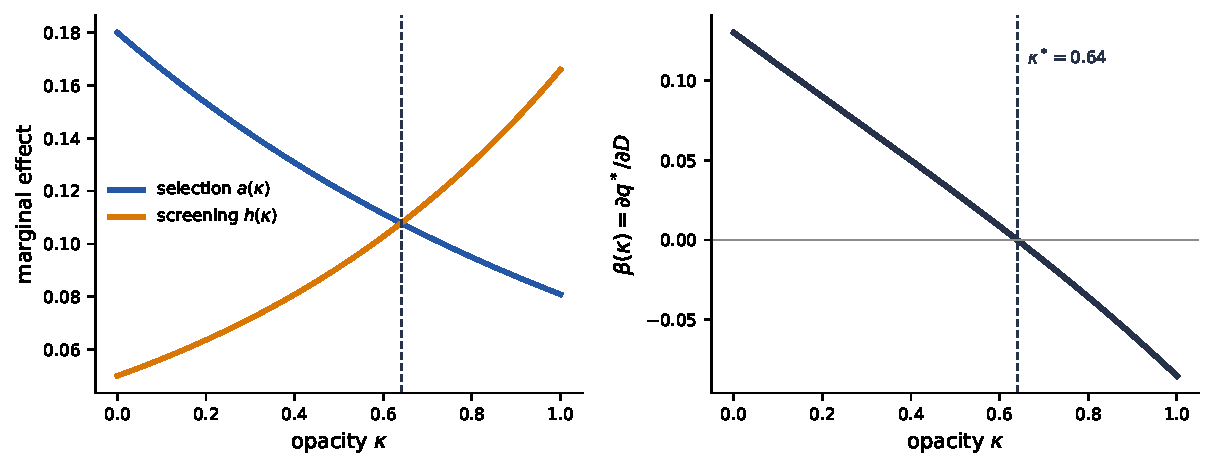
\includegraphics[width=\linewidth]{../code/figures/opacity_threshold.pdf}
  \end{columns}
\end{frame}

\begin{frame}{3 · From origination quality to future delinquency}
  Let future observed delinquency satisfy
  \[
    m_{j,s,t+h}=\rho_h q^*_{j,s,t}+\varepsilon_{j,s,t+h},
    \qquad \rho_h>0.
  \]
  Then
  \[
    \operatorname{sign}\left(
    \frac{\partial\mathbb E_t[m_{j,s,t+h}]}{\partial D_{j,s,t}}
    \right)
    =\operatorname{sign}[a(\kappa_s)-h(\kappa_s)].
  \]
  \vspace{0.7em}
  \begin{itemize}
    \item \(D\) is computed within product, maturity, currency, and month.
    \item \(\kappa_s\) is an ordinal segment-opacity proxy, not a directly
          estimated structural primitive.
    \item The empirical exercise compares out-of-sample forecasts.
  \end{itemize}
\end{frame}

\begin{frame}{4 · Why this is not already solved}
  \small
  \begin{tabular}{@{}p{0.20\textwidth}p{0.31\textwidth}p{0.39\textwidth}@{}}
    \toprule
    Paper & What it solves & What remains here \\
    \midrule
    Varian (1980) & Shoppers, captive buyers, price dispersion & No screening or default \\
    Broecker (1990) & Imperfect tests and rate competition & Test technology is not an effort choice \\
    Ruckes (2004) & Endogenous screening over the business cycle & No opacity threshold for the relative-price signal \\
    Dell'Ariccia and Marquez (2006) & Screening versus pooling under interbank information asymmetry & No continuous \(\partial q^*/\partial D\) decomposition \\
    \bottomrule
  \end{tabular}
  \vspace{0.7em}
  Checked: model sections and appendices, the accessible working-paper record,
  and the full IMF reprint.
\end{frame}

\begin{frame}{5 · Proof, simulation, and Lean plan}
  \begin{enumerate}
    \item \textbf{Proof:} Proposition 1, then a robustness result for general
          increasing \(R(D)\).
    \item \textbf{Simulation:} map the parameter region where \(a-h\) crosses
          zero and verify interiority and probability bounds.
    \item \textbf{Forecasting:} evaluate whether \(D\) improves predictions of
          \(m_{t+h}\) by segment opacity and horizon.
    \item \textbf{Lean:} formalize the threshold theorem after its assumptions
          and statement are frozen.
  \end{enumerate}
  \vspace{0.5em}
  Already checked in code: FOC, SOC, monotonicity, unique crossing, effort
  bounds, and \(q^*\in(0,1)\).
\end{frame}

\begin{frame}{5 · Main risk and disciplined fallback}
  \begin{block}{Most likely failure}
    The maintained condition \(h'(\kappa)>0\) may fail in a richer signal
    technology or in calibration.
  \end{block}
  \begin{block}{Fallback result}
    Do not force a reversal. Characterize the three identified regions
    \[
      a(\kappa)>h(\kappa),\qquad
      a(\kappa)=h(\kappa),\qquad
      a(\kappa)<h(\kappa),
    \]
    and treat threshold existence as an estimable restriction.
  \end{block}
  \vfill
  \centering
  \Large
  The contribution is the \alert{condition for the sign}, not a guaranteed
  negative coefficient.
\end{frame}

\end{document}
